\section{Results and Analysis}

\subsection{Accuracy and Model Behavior}
The model enforces the constraint \( S + I + R = 1 \) at every grid cell and time step, ensuring physical consistency and mitigating numerical drift due to floating-point errors. This is achieved via post-integration normalization.

Across all scenarios, the model exhibits expected qualitative behaviors:
\begin{itemize}
    \item \textbf{Higher \( \beta \)}: Faster and broader propagation; earlier infection peaks
    \item \textbf{Higher \( \gamma \)}: Rapid decline in infections; quicker recovery
    \item \textbf{Low \( \beta + \gamma \)}: Slower dynamics; longer persistence of initial state
\end{itemize}

These trends confirm that the simulation is sensitive to parameters and effectively captures distributed information and congestion dynamics.

\subsection{Visualization}

\subsubsection{Global SIR Evolution}
We first provide an overview of the global trends of the SIR variables:
\begin{figure}[H]
    \centering
    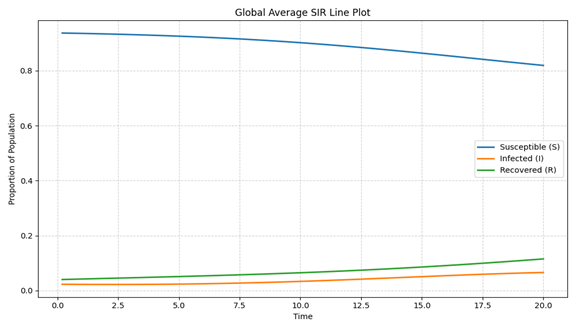
\includegraphics[width=14cm]{Images/pic5.png}
    \caption*{Shows the global average values of Susceptible (S), Infected (I), and Recovered (R) over time, plotted as line graphs. It confirms the expected dynamics: S steadily decreases, while I and R gradually increase.}
    \label{fig:sir_line_plot}
\end{figure}

\begin{figure}[H]
    \centering
    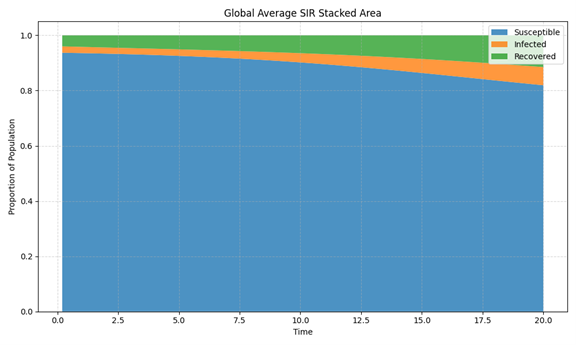
\includegraphics[width=14cm]{Images/pic6.png}
    \caption*{Presents the same data in the form of a stacked area chart, emphasizing the total population conservation (S + I + R = 1) and the proportion each state occupies throughout the simulation.}
    \label{fig:pic6}
\end{figure}


\subsubsection{Per-Rank Behavior}
Because the simulation is distributed across MPI processes, it is important to visualize the behavior of each rank individually.
\begin{figure}[H]
    \centering
    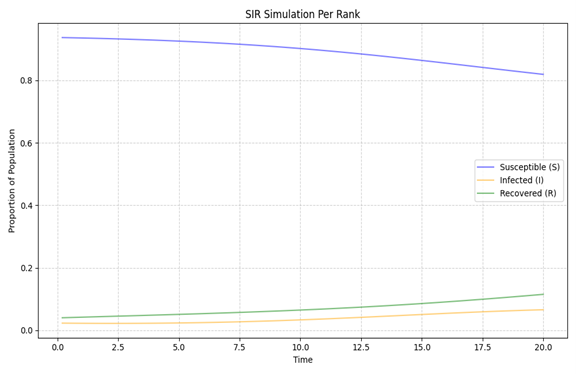
\includegraphics[width=14cm]{Images/pic7.png}
    \caption*{Displays the evolution of S, I, and R within each MPI rank using line plots. These trends reveal differences in infection dynamics between regions, reflecting the spatial heterogeneity.}
    \label{fig:sir_line_plot}
\end{figure}

\subsubsection{Infection Propagation and Peak Timing}
To analyze the infection wave’s temporal spread and communication among ranks:
\begin{figure}[H]
    \centering
    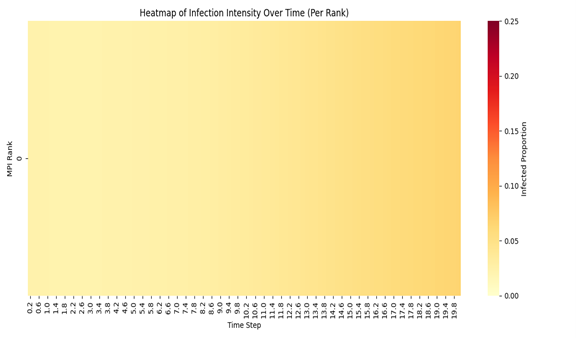
\includegraphics[width=14cm]{Images/pic8.png}
    \caption*{This is a heatmap that illustrates the infection intensity per rank over time. It demonstrates how the infection begins locally and gradually spreads to other ranks through the ghost cell exchange mechanism.}
    \label{fig:sir_line_plot}
\end{figure}

\subsection{Performance and Scaling Analysis}
Based on the results presented in Section 7.2, we evaluate the parallel simulation’s computational efficiency. The recorded timing logs, including phase-specific breakdowns and rank-level measurements, confirm that the workload is well-balanced across MPI processes. Most of the execution time is spent in the local computation phase, while communication costs remain relatively low due to the use of non-blocking MPI operations.


The distribution of timing across ranks shows minimal variability, indicating that the domain decomposition strategy (divideIntoOptimalBlocks) effectively assigns cells to processes with balanced loads. The asynchronous communication scheme using MPI\_Isend and MPI\_Irecv overlaps well with computation, helping to reduce idle time during ghost cell exchange.

